\section{Results}
\label{sec:results}
Over the next sections I present the main results of my experiment to support our claim that SafraFT is correct, to show how SafraFT compares to SafraFS and to exemplify the performance of SafraFT under the presence of faults.

The observations are based on runs of the system described in \cref{sec:methods} on the DAS-4 cluster at the Vrije Universiteit of Amsterdam.
I meassured runs on networks from 50 to 2000 nodes for SafraFT and SafraFS.
SafraFT was also tested with 1 to 5 nodes failing per run (dubbed 5n) and with 90\% node failure.
\cref{table:runs} presents how many repetition of each configuration were run.

The raw data including a manual how to interpret it can be found TODO here.
\begin{table}[]
	\centering
	\begin{tabular}{@{}lllll@{}}
		\toprule
		Algorithm & Network              & Faults & Repetitions  & \#Instances / DAS-4 node   \\ \midrule
		SafraFS   & 50                   & 0      & 100          & 25                    \\
		SafraFS   & 250/500/1000/2000    & 0      & 100          & 125                   \\
		SafraFT   & 50                   & 0      & 100          & 25                    \\
		SafraFT   & 250/500/1000/2000    & 0      & 100          & 125                   \\
		SafraFT   & 50                   & 5n     & 100          & 25                    \\
		SafraFT   &    250/500/1000/2000 & 5n     & 100          & 125                   \\
	    SafraFT   & 50                   & 90\%   & 100          & 25                    \\
		SafraFT   &    250/500/1000/2000 & 90\%   & 100          & 125                   \\ \bottomrule
	\end{tabular}
	\caption{List of all configurations run. Per physical DAS-4 node with 8 cores multiple virtual instances in their own processes where run (columm '\#Instances / DAS-4 node`). The amount of physical node equates to network size divided by instances.}
	\label{table:runs}
	% TODO include number of nodes and number of instances per node
\end{table}

\subsection{Correctness of SafraFT}
\label{ssec:correctness}
The experiment is aimed to support our paper with a practical, correct application of our alogorithm.
Towards this goal I build multiple correctness checks into the experiment. 

To assure nothing happens after termination detection, the application logs if any messages are received or actions are executed after termination has been detected and announced. 
The analysis tools provided with the experiment point these logs out to make sure they are not overlooked.

To proof termination is not detected to early, I use offline analysis (see \cref{ssec:offline-analysis}) to determine the point of actual termination and verify that detection happened after.
All % TODO runs using SafraFT under the presence of faults confirm that termination was never detected to early according to this framework.

However, the experiment revealed that the framework for termination chosen to develop SafraFT is not complete and does not cover all cases for my experiment setup.
SafraFT is developed for the following and commonly used definition of termination:
\begin{enumerate}
	\item All nodes are passive
	\item No messages are in the channels
\end{enumerate}
This definition is based on the fact that a node is either an initiator or can only become active if it receives a message. 
However, under the presence of failures and if additionally the outcome of the algorithm depends on the set of alive nodes, nodes might get activated by the detection of a failure.
For example, when Chandy Misra builds a sink tree, nodes that detect a crash of their parents will become active afterwards to find a new path towards root.
The idea described above leads to the following concrete scenario: lets consider the situation that all node are passive and no message are in the channel. 
In other words, the system terminated by our definition.
Node \co{X} forwards the token and crashes afterwards. 
Node \co{Y} calls announce after receipt of the token.
Assume node \co{Z} is a child of \co{X} and detects the crash of its parent, it becomes active after termination has been formally reached and announced.
By sending out \co{REQUEST} message, it might activate other nodes again.

To conclude, the definition of termination that our algorithm is build upon does not fully capture our choice of basic algorithm which could lead to an early detection of termination.

To verify if situations like this actual occur during the experiment, I analysed the logs generated according to both defintions of termination - the one used to develop SafraFT and the same definition but extended with the assumption that termination is postponed until the last crash leading to activity in the basic algorithm has been detected.

As stated above, SafraFT did never detect termination too early according to the first definition.
According to the extended definition it detects termination to early in %TODO out of % TODO runs.
However, due to fact that repairing the sink tree after detecting a parent crash is quite fast and there is a short time window to do so while the announce call propagates to all nodes only in % TODO of these cases that leads to the situation that basic activity happened after detected
termination.

I carefully reviewed each repetition in which termination is detected too early according to the extended definition to verify that early termination detection is in fact caused by a situation as described above.
The logs of these runs provide a summary of all detections of parent crashes close to the announce call to ease this procedure.

\subsection{Comparision of Safra versions}
This section compares SafraFS and SafraFT. 
Additionally, it analysis how the network size influences both algorithms.

The number of tokens send in total and after termination is presented in \cref{fig:tokens-and-tokens-after}.

\begin{sidewaysfigure}[ht]
	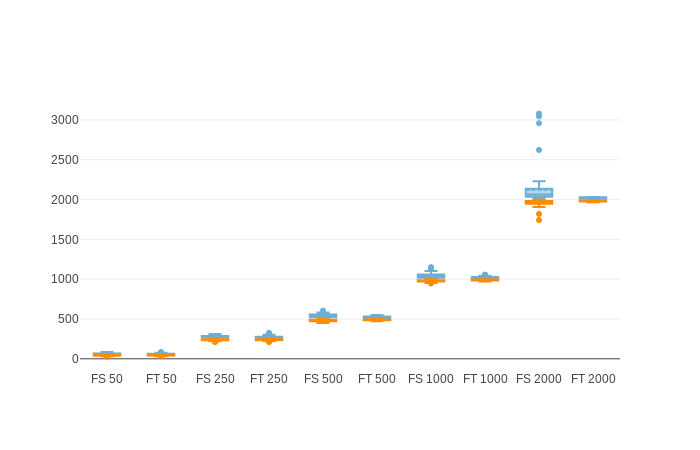
\includegraphics{figures/tokens-and-tokens-after.png}
	\caption{Tokens (blue) and tokens after termination (orange) for SafraFT and SafraFS in fault free runs for all network sizes.}
	\label{fig:tokens-and-tokens-after}
\end{sidewaysfigure}

The key observation is that SafraFS and SafraFT behave highly similiar.
Nonetheless, there are small differences.
SafraFT sends slightly less tokens.
The biggest difference is around 30 tokens out of roughly 1000 tokens for a network with the size of thousand.
% TODO results for 2000
Also the results for SafraFS show a slightly higher variance.
Most likely these differences are caused by implemenation details and not generalizable.

As one would expect, the number of tokens grows linearly with the network size.
Note that the first network size is 5 times smaller than the second for bigger networks the  size doubles for each run.

The bit complexity of SafraFS is constant.
In this experiment each token of SafraFS contains 12 bytes.
SafraFT has a bit complexity linearly to the network size (when no faults occur).
For a network of 50 nodes each token has 420 bytes; a token in a 2000 node network counts 16020 bytes.
The growth can be described by $bytes = 8 * <network size> + 20$.

I measured two kinds of timing metrics in this experiment.
On the one hand, there are the wall time metrics of total time and total time after termination.
Both were recorded in elapsed seconds between two events. 
These events are start of the Safra and basic algorithm until each instance is informed of termination for total time. 
Total time after termination is defined as the ammount of seconds between the actual termination (extended termination definition from \cref{ssec:correctness}) and the event of an node calling
announce. % TODO is that too much explanation, does everybody but you know so?
On the ohter hand, there are basic, Safra and Safra after termination processing times (including the time needed to send of messages).
These are the accumulated times all instances needed to process basic or Safra functionality.
Total times and processing times are measured in a different way and should not be compared directly for multiple reasons. 
First, while total times include idle times, time spent for logging (where the process did not execute or methods), processing time do not include these.
Secondly, total time is wall time between two events and processing times are accumulated over all processes. 
One particular example for when this leads to differences is that time spent concurrently by two processes counts double in processing time metrics but only once in wall time metrics.

\begin{table}
	\centering
	\begin{tabular}{rrrrrr}%
		\toprule
		\multicolumn{1}{c}{Network} &
		\multicolumn{1}{c}{Basic} &
		\multicolumn{1}{c}{Safra FS} &
		\multicolumn{1}{c}{Overhead FS} &
		\multicolumn{1}{c}{Safra FT} &
		\multicolumn{1}{c}{Overhead FT} \\
		\midrule
		\csvreader[head to column names]{figures/processing-times.csv}{}
		{\\\networkSize & \basic & \FS & \FSoverhead \% & \FT & \FToverhead \%}
		\\\bottomrule
	\end{tabular}
	\caption{Total processing times and processing times after termination (in braces) in seconds and overhead caused by processing Safa's methods in percent}
	\label{table:processing-times}
\end{table}
% TODO add percent sign to overhead numbers

One can observe in \cref{table:processing-times} that SafraFT uses more processing time than SafraFS and much of this time is spent between actual termination and termination detection.
Furthermore, one sees that SafraFS times grow less  than SafraFT times with increasing networks.z
This hints for a change in time complexity between the two versions.

A small subexperiment of excluding the time spent to send messages from the processing time revealed that most of this difference can be tributed to writting tokens onto the wire.
As we know from a previous paragraph, the number of token send does not differ between the algorithms.
Therefore, I believe that these differences are caused by the higher bit complexity of SafraFT. 
This would explain the total increase in the timing from SafraFS to SafraFT, as well as, the change of time complexity.
The time complexity would change because the increase in network size leads to more token being sent (as in SafraFS) but also to bigger tokens being sent.

The difference in processing time spent after termination is higher than the difference in total processing time.
The first reason for this is that most tokens are sent after termination (see \cref{fig:tokens-and-tokens-after}).
A second reason is that much of the total processing time is spent in the methods handling receive and sending of basic messages because they are called that often.
These do not change that significantly between both Safra versions.
Hence, the increase of processing time to send tokens shows less in the total times.

The processing time \cref{table:processing-times} also presents a comparision of the time spent for the basic algorithm and both Safra versions.
Although, SafraFT uses significantly more time, the overhead on the processing time stays moderate with a maximum of % TODO percent
\\
\begin{table}
	\centering
	\begin{tabular}{rrrrrrr}%
		\toprule
		\multicolumn{1}{c}{Network} &
		\multicolumn{1}{c}{Safra FS} &
		\multicolumn{1}{c}{Safra FT} &
		\multicolumn{1}{c}{$\Delta$} &
		\multicolumn{1}{c}{Safra FS after} &
		\multicolumn{1}{c}{Safra FT after} &
		\multicolumn{1}{c}{$\Delta$}  \\
		\midrule
		\csvreader[head to column names]{figures/total-times.csv}{}
		{\\\networkSize & \FS & \FT & \difference & \FSAfter & \FTAfter & \differenceAfter}
		\\\bottomrule
	\end{tabular}
	\caption{Wall times total and after termination for SafraFT and SafraFS in seconds with ratios}
	\label{table:total-times}
\end{table}

The same pattern of SafraFT using more time and reacting stronger to an increase in network size is visible for total times in \cref{table:total-times}.
An exception from this pattern is the strong rise of total time for SafraFT in networks with 250 nodes.
% TODO might be because of?

For SafraFS roughly half of the time is spent after termination for small networks.
In big networks the part of time spent after termination is lower because the fraction spent by the basic algorithms becomes dominant. 

The systems using SafraFT spent the majority of their time to detect termination because of the already noted higher time complexity.

I would like to note that the low processing time overhead of Safra is not in contradiction to the large amount of wall time spent after termination.
These seemingly opposing results arise from the difference between wall time and processing time: the basic algorithm is much more active in the beginning that is when it accumulates a lot of processing time; while Safra causes a lot of idle time at the end when all processes wait for their predecessor to pass on the token. 
This idle time is not included in processing time but wall time does include it.

To conclude, the experiments confirm that the message complexity of SafraFT remains as for the fault sensitive version but its higher bit complexity causes a higher time complexity which leads to a later termination detection. 
Still, SafraFT causes only a moderate processing time overhead between %TODO.


\subsection{Influence of faults}
In the following paragraphs, I present and explain the data generated by runs under the presence of node crashes.
I run to highly different scenarios: one considering networks with 1 to 5 nodes failing and one with 90\% of all nodes crashing.
These scenarios are chosen to show SafraFT in both the realistic case of a low number of faults to handle, as well as, the an extreme case; with the aim to confirm that SafraFT handles both cases correctly and without unreasonable deterioration in any metric.

% TODO token size is missing
\subsubsection{Tokens}
\label{ssec:tokens-faulty}
For both the networks where between 1 and 5 nodes failed, as well as, for the highly faulty runs with 90\% node failure, the number of tokens increased compared to runs without any faults.
More so for highly faulty networks more faults. The data is presented \cref{fig:tokens-and-tokens-after-faulty} and \cref{table:tokens-faulty}. % Table presents comparision with 0 configuration

\begin{sidewaysfigure}[ht]
	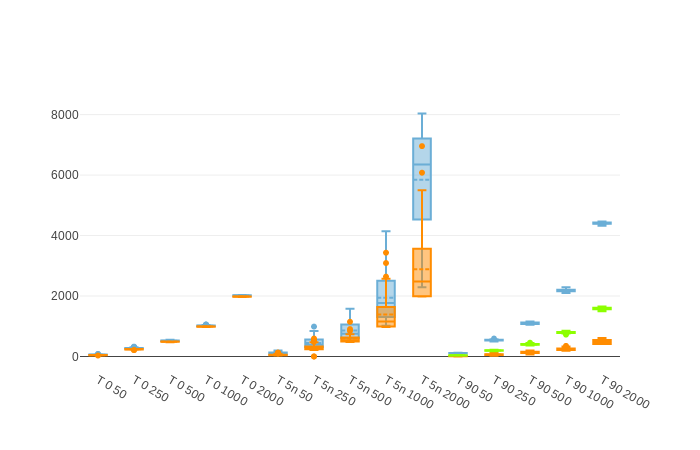
\includegraphics{figures/tokens-and-tokens-after-faulty.png}
	\caption{Tokens (blue) and tokens after termination (orange) for SafraFT on the x-axis for 5 network sizes and 5n and 90\% fault configurations on the y-axis.		Backup tokens in green, shown only for 90\%}
	\label{fig:tokens-and-tokens-after-faulty}
\end{sidewaysfigure}

\begin{table}
	\centering
	\begin{tabular}{rrrrrr}%
		\toprule
		\multicolumn{1}{c}{Network} &
		\multicolumn{1}{c}{No faults} &
		\multicolumn{1}{c}{5n} &
		\multicolumn{1}{c}{$\Delta$} &
		\multicolumn{1}{c}{90\%} &
		\multicolumn{1}{c}{$\Delta$} \\
		\midrule
		\csvreader[head to column names]{figures/tokens-faulty.csv}{}% use head of csv as column names
		{\\\networkSize & \noFaults & \fiveN & \differenceFiveN & \ninety & \differenceNinety}
		\\\bottomrule
	\end{tabular}
	\caption{Tokens before and after termination (in braces). For different fault scenarios compared to fault-free networks.}
	\label{table:tokens-faulty}
\end{table}

Otherwise, the two types of fault simulation had a highly different influence on the tokens and tokens after termination metrics.

Between 1 and 5 node failures lead to a strong increase in the variance of tokens sent, as well as, tokens sent after termintaion.
This seems reasonable as runs with failing node might lead to more different situations as runs without fails e.g. one failing node could easily cause an extra token when it leads to an backup token being issued and forwarded (this token is marked black until for a whole run), at the same time, a single failing node that is a leaf in a Chandy Misra sinke tree and that crashes just before the call of announce at the successor  causes no further activity.
The same example provides an idea why the variability increases in big networks. 
That is because one extra round in a big network has a much higher impact on the token count than in a small network.

The phenomenon explained in the last paragraph most likely causes the extremely high maximum of tokens sent and overlinear increase of the average number of tokens in networks with 2000 nodes for 1 to 5 nodes failing.

Other than networks with one to 5 failing nodes, networks with up to 90\% node failure lead to a similiar variance in tokens and tokens after termination as a fault free networks.
A likely explanation is that the low survival rate of 1 out of 10 instances leads to less different scenarios than in the fault scenario treated the last paragraphs e.g. for a network size of thousand roughly 995 nodes survived for 5n but only 100 nodes survive in the runs discussed in this paragraph.

Even though, only one 10th of the nodes survive to participate in the latter token rounds, the highly faulty networks produced more tokens than any other network of the same size.
That is most likely due to the high amount of backup tokens generated (also shown in \cref{fig:tokens-and-tokens-after-faulty})

Different from all other networks, highly faulty networks exhibit a much lower token to token after termination ratio caused by the low number of nodes alive in the last rounds.
    
\subsubsection{Backup tokens}
The average amount of backup tokens sent for either fault simulation and every network size is lower than the number of faults.
This is because SafraFT only issues backup tokens when the fault of its successor is detected via the fault detector but not if this fault is noticed by receiving a token.
That result is suprising because the simulated fault detector in my setup detects faults in a really timely manner.
Still, there are some runs were 1 to 5 nodes fail but no backup token is issued even for really big networks. 

The other extreme were more backup tokens are issued than faults occure exists as well.
This can be explained by my decission to have node failing after issuesing a backup token.
For example, nodes \co{A}, \co{B} and \co{C} follow each other in the ring, node \co{C} fails which is detected by \co{B} and a backup token is issued.
After, issueing the backup token \co{B} fails on detection \co{A} issues a backup token towards \co{C}.
Only then \co{A} detects the failing of \co{C} and issues a second backup token to its new successor.  


\subsubsection{Processing Time}
The observations of this chapter are backed by \cref{table:processing-times-faulty}.

As for tokens, one can see an increase in processing times before termination under the presents of faults compared to fault free runs. 
This increase is stronger for runs with more faults.
Which is no surprise as these runs also produced more tokens.

For runs with 1 to 5 failing node a higher variability in the processing times before and after termination becomes apparent. 
Most likely this is because of the higher diversity of scenarios possible if some nodes fail  as explained in \cref{ssec:tokens-faulty}.
As the processing time grows for this runs, so does the processing time after termination.

For highly faulty networks one observes results in line with the results for tokens in these networks.
The variability for processing time before or after termination is not raised compared to fault free networks.
The processing time taken is even higher than the one for less faulty networks.

Less processing time after termination is spent than for fault free networks because less tokens need to be send.
% TODO transpose these tables
\begin{table}
	\centering
	\begin{tabular}{rrrrrr}%
		\toprule
		\multicolumn{1}{c}{Network} &
		\multicolumn{1}{c}{No faults} &
		\multicolumn{1}{c}{5n} &
		\multicolumn{1}{c}{$\Delta$} &
		\multicolumn{1}{c}{90\%} &
		\multicolumn{1}{c}{$\Delta$} \\
		\midrule
		\csvreader[head to column names]{figures/processing-times-faulty.csv}{}
		{\\\networkSize & \noFaults & \fiveN & \differenceFiveN & \ninety & \differenceNinety}
		\\\bottomrule
	\end{tabular}
	\caption{Processing times before and after termination (in braces) in seconds. For different fault scenarios compared to fault-free networks.}
	\label{table:processing-times-faulty}
\end{table}
    
 \subsection{Total time}
 In line with the observations from the two sections before, one observes:
 \begin{itemize}
 	\item an increase in total time spent which is more pronounced on more faulty networks
 	\item a higher variability for time spent before and after termination for less faulty networks
 	\item less time spent after termination by highly faulty networks
 \end{itemize}
 The absolute numbers and relative increases are presented in \cref{table:total-times-faulty}.
 
 \begin{table}
 	\centering
 	\begin{tabular}{rrrrrr}%
 		\toprule
 		\multicolumn{1}{c}{Network} &
 		\multicolumn{1}{c}{No faults} &
 		\multicolumn{1}{c}{5n} &
 		\multicolumn{1}{c}{$\Delta$} &
 		\multicolumn{1}{c}{90\%} &
 		\multicolumn{1}{c}{$\Delta$} \\
 		\midrule
 		\csvreader[head to column names]{figures/total-times-faulty.csv}{}
 		{\\\networkSize & \noFaults & \fiveN & \differenceFiveN & \ninety & \differenceNinety}
 		\\\bottomrule
 	\end{tabular}
 	\caption{Total times before and after termination (in braces) in seconds. For different fault scenarios compared to fault-free networks.}
 	\label{table:total-times-faulty}
 \end{table}
 
 % TODO why does total time after for less faulty networks not increase.
 % TODO why are these increases and not other to be expected and reasonable






	
